% ============================================================================
\section{Introduction}
\label{sec:intro}
% ============================================================================

Multi-teacher on-policy distillation (MOPD) merges several specialist teachers
into one student. The student samples a response, the teacher for that task
scores every token, and the student is updated to reduce the sampled-token
reverse KL to the teacher \citep{ma2026mopdmultiteacheronpolicydistillation}.
Every MOPD method must choose a task mixture, and the choice matters more than
it looks. Open-MOPD reports that, under token-mean aggregation, a $25\times$
difference in response length leaves instruction following with about $1\%$
of the gradient tokens despite $20\%$ of the prompts
\citep{gao2026openmopddiagnosingfixingcapability}. D$^3$-MOPD adapts the
mixture online from the teacher-loss gap and its descent rate
\citep{sun2026d3mopd}. In both cases the mixture is at once the training
objective and the compute schedule, so a change in one cannot be separated
from a change in the other.

We keep the two apart. The objective is a weighted sum of per-task teacher
losses with weights chosen before training. Each optimizer step accumulates
$G$ fixed-size micro-batches, each drawn from a single task, and the only
online decision is how many micro-batches each task gets. Multiplying each
micro-batch loss by its task weight divided by its task's count makes the
expected gradient identical under every allocation
(Section~\ref{sec:setting}). The allocation therefore decides only how
precisely each task gradient is estimated, and the natural criterion is
variance: spend more micro-batches where the gradient is noisier.
\missing{In our four-teacher run the per-micro-batch gradient noise, measured
in AdamW coordinates, differs by up to X$\times$ across tasks and drifts by
Y$\times$ over training (Figure~\ref{fig:allocation_dynamics}), so no fixed
split is variance-optimal throughout.}

\begin{figure}[t]
    \centering
    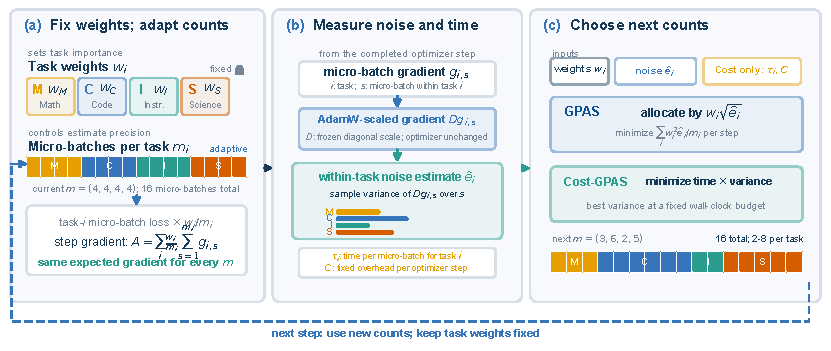
\includegraphics[width=\linewidth]{figures/gpas_main_figure.pdf}
    \caption{GPAS fixes the objective weights $w$ and adapts only the
    micro-batch counts $m$. Gradients from the completed step give each task's
    noise in AdamW coordinates, and measured time adds the cost correction, so
    the next allocation needs no additional model passes.}
    \label{fig:gpas_overview}
\end{figure}

Gradient-Preconditioned Adaptive Sampling (GPAS) assigns task $i$ a count
proportional to $w_i\sqrt{e_i}$, where $w_i$ is its weight and $e_i$ its
per-micro-batch gradient noise measured after AdamW's diagonal scaling. This
is the classical stratified-sampling rule, which samples each stratum in
proportion to its standard deviation, applied in the coordinates the optimizer
actually uses. The coordinates matter: raw and scaled noise can rank tasks
differently, and allocating by raw noise can then increase the variance that
AdamW sees (Section~\ref{sec:theory}). Cost-GPAS additionally uses the
measured time per micro-batch and the fixed time per step, so that variance is
minimized per GPU hour instead of per step. Both rules run on statistics from
the step just completed, namely each task's within-step gradient variance and
its timing. Every task is present in every step, so these statistics are
always available, and computing them needs one parameter-sized buffer and no
extra forward or backward pass. GPAS is a drop-in change to a standard MOPD
trainer with AdamW.

\missing{Findings, to be written from the four-teacher runs: (i) how much the
scaled noise levels differ across tasks and drift, and in what fraction of
steps raw and scaled noise rank the tasks differently; (ii) the held-out
teacher-loss reduction of GPAS at matched steps; (iii) the GPU-hour saving of
Cost-GPAS at Uniform's final loss; (iv) per-task downstream results relative
to Uniform.}

Our contributions are:
\begin{itemize}
    \item a fixed-objective MOPD estimator in which adaptive micro-batch
    counts change the variance of the gradient estimate but not its
    expectation;
    \item GPAS and Cost-GPAS, optimizer-aware count rules whose statistics
    come from the passes MOPD already performs;
    \item a four-teacher study of Qwen3-1.7B that measures noise and
    allocation dynamics, held-out loss per step and per GPU hour, and
    per-task downstream capability, with the recipe and logs released.
\end{itemize}
